

\documentclass[12pt]{article}
\usepackage{amsmath}
\usepackage{latexsym}
\usepackage{amsfonts}
\usepackage[normalem]{ulem}
\usepackage{array}
\usepackage{amssymb}
\usepackage{graphicx}
\usepackage[backend=biber,
style=numeric,
sorting=none,
isbn=false,
doi=false,
url=false,
]{biblatex}\addbibresource{bibliography.bib}

\usepackage{subfig}
\usepackage{wrapfig}
\usepackage{wasysym}
\usepackage{enumitem}
\usepackage{adjustbox}
\usepackage{ragged2e}
\usepackage[svgnames,table]{xcolor}
\usepackage{tikz}
\usepackage{longtable}
\usepackage{changepage}
\usepackage{setspace}
\usepackage{hhline}
\usepackage{multicol}
\usepackage{tabto}
\usepackage{float}
\usepackage{multirow}
\usepackage{makecell}
\usepackage{fancyhdr}
\usepackage[toc,page]{appendix}
\usepackage[hidelinks]{hyperref}
\usetikzlibrary{shapes.symbols,shapes.geometric,shadows,arrows.meta}
\tikzset{>={Latex[width=1.5mm,length=2mm]}}
\usepackage{flowchart}\usepackage[paperheight=11.0in,paperwidth=8.5in,left=1.0in,right=1.0in,top=0.75in,bottom=0.75in,headheight=1in]{geometry}
\usepackage[utf8]{inputenc}
\usepackage[T1]{fontenc}
\TabPositions{0.5in,1.0in,1.5in,2.0in,2.5in,3.0in,3.5in,4.0in,4.5in,5.0in,5.5in,6.0in,}

\urlstyle{same}


 %%%%%%%%%%%%  Set Depths for Sections  %%%%%%%%%%%%%%

% 1) Section
% 1.1) SubSection
% 1.1.1) SubSubSection
% 1.1.1.1) Paragraph
% 1.1.1.1.1) Subparagraph


\setcounter{tocdepth}{5}
\setcounter{secnumdepth}{5}


 %%%%%%%%%%%%  Set Depths for Nested Lists created by \begin{enumerate}  %%%%%%%%%%%%%%


\setlistdepth{9}
\renewlist{enumerate}{enumerate}{9}
		\setlist[enumerate,1]{label=\arabic*)}
		\setlist[enumerate,2]{label=\alph*)}
		\setlist[enumerate,3]{label=(\roman*)}
		\setlist[enumerate,4]{label=(\arabic*)}
		\setlist[enumerate,5]{label=(\Alph*)}
		\setlist[enumerate,6]{label=(\Roman*)}
		\setlist[enumerate,7]{label=\arabic*}
		\setlist[enumerate,8]{label=\alph*}
		\setlist[enumerate,9]{label=\roman*}

\renewlist{itemize}{itemize}{9}
		\setlist[itemize]{label=$\cdot$}
		\setlist[itemize,1]{label=\textbullet}
		\setlist[itemize,2]{label=$\circ$}
		\setlist[itemize,3]{label=$\ast$}
		\setlist[itemize,4]{label=$\dagger$}
		\setlist[itemize,5]{label=$\triangleright$}
		\setlist[itemize,6]{label=$\bigstar$}
		\setlist[itemize,7]{label=$\blacklozenge$}
		\setlist[itemize,8]{label=$\prime$}



 %%%%%%%%%%%%  Header here  %%%%%%%%%%%%%%


\pagestyle{fancy}
\fancyhf{}
\chead{ \chapter{\  }}
\renewcommand{\headrulewidth}{0pt}
\setlength{\topsep}{0pt}\setlength{\parindent}{0pt}

 %%%%%%%%%%%%  This sets linespacing (verticle gap between Lines) Default=1 %%%%%%%%%%%%%%


\renewcommand{\arraystretch}{1.3}
\font\myfont=cmr12 at 40pt

\title{{\myfont Victim Cache and Skewed Associative Cache}}
\date{}


%%%%%%%%%%%%%%%%%%%% Document code starts here %%%%%%%%%%%%%%%%%%%%



\begin{document}

\maketitle
\par

\chapter{31.10.2019}\par

{\fontsize{18pt}{21.6pt}\selectfont \textbf{─}}

{\fontsize{16pt}{19.2pt}\selectfont \textcolor[HTML]{008575}{Group Members}\par}\par

Ayush Mangal (18114016)\par

Harshit Verma (18114029)\par

Hemant (18114030)\par

Hemil Panchiwala (18114031)\par

Kunal Mohan (18116042)\par

Nalin Prabhath (18116015)\par

Piyush Gupta (18116059)\par
\pagebreak
{\fontsize{24pt}{28.8pt}\selectfont \uline{Abstract}\par}\par
\par
In our project, we have compared two new types of cache - the Skewed Associative Cache and Victim Cache. \par

Skewed Associative Cache has better behaviour than Set-associative caches. Typically a two-way skewed-associative cache has the hardware complexity same as that of two-way set-associative cache, yet simulations show that it exhibits approximately the same hit ratio as a four-way set-associative cache of the same size. \par

Victim Cache is basically a fully associative cache, comparatively smaller in size than L1 cache and placed behind the L1 cache. It holds the evicted block because of conflict miss from L1 cache. So rather than evicting the memory block, we store it in another cache, thus increasing the hit ratio and increasing the speed.\par


\vspace{\baselineskip}
\setlength{\parskip}{8.04pt}
{\fontsize{24pt}{28.8pt}\selectfont \textbf{\uline{Importance}}}\par}\par

\parbox{\linewidth}{As hardware architecture and technology advanced, processor performance grew much faster than memory cycle times, leading to a large gap in performance. The problem of increasing memory latency, relative to processor speed, has been dealt with by adding high-speed cache memory.}}\par

\parbox{\linewidth}{Performance of associative caches depends on the associativity of the cache. There is a continuous trade-off between the access time and the hit ratio depending on the associativity. Skewed associative caches are better than set-associative cache because they have access time equivalent to that of a 2-way set-associative cache but the hit ratio is similar to that of a 4-way set-associative cache.}}\par

Direct Mapped caches have faster access time than \href{https://en.wikipedia.org/wiki/Set-associative}{set-associative} caches. However, for a direct-mapped cache if multiple cache blocks in the memory map to the same cache-line they end up evicting each other when any one of them is accessed. This is known as the cache conflict problem. This problem is resolved by increasing the associativity of the cache. But there is a limit to which associativity can be increased owing to the complexity in its implementation. Thus, for solving the cache conflict problem for a cache with limited associativity, victim cache is employed.}\par


\vspace{\baselineskip}
{\fontsize{30pt}{36.0pt}\selectfont \uline{Description}}\par}\par


\vspace{\baselineskip}
{\fontsize{24pt}{28.8pt}\selectfont \textbf{\uline{Victim Cache}}\par}\par


\vspace{\baselineskip}
A victim cache is a small, usually fully associative cache placed in the refill path to CPU cache, and it stores all the blocks evicted from that level of cache.\par

Victim cache is a hardware technique to improve performance of caches. It decreases conflict misses and improve hit latency. It is employed at the refill path of Level 1 cache, such that any cache line gets evicted from the cache is cached in the victim cache. Thus, victim cache gets populated only when data is pushed out of L1 cache.\par

In case of a miss in L1 cache, the victim cache is searched for the data. If the resulting access is a hit, the contents of L1 cache-line and the matching victim cache are swapped.\par

\setlength{\parskip}{3.96pt}
{\fontsize{14pt}{16.8pt}\selectfont \uline{Implementation}\par}\par

\setlength{\parskip}{8.04pt}
The behavior of a victim cache in its respective interaction with the corresponding level cache is given below:\par

\textbf{\uline{Cache Hit:}} No action\par

\textbf{\uline{Cache Miss, Victim Hit:}} Block in victim cache and the one in L1 cache are replaced. This new entry in L1 cache becomes the most recently accessed block.\par

\textbf{\uline{Cache Miss, Victim Miss:}} The block is brought from next level (L2 cache in our implementation). The block evicted from L1 cache is stored in victim cache.\par

\textbf{Example-}\par

\setlength{\parskip}{5.04pt}
Suppose a direct-mapped L1 cache with blocks A, B pointing to the same set. It is linked to a 2 entry fully associative victim cache with blocks C, D in it.\par

The trace to be followed: A, B, A, B$ \ldots $ \par

From the screenshot, we can see that, in the case of victim cache (VC) hit, blocks A and B are swapped. The least recently used block of VC remains as it is. Hence, it gives an illusion of associativity to the direct-mapped L1 cache, in turn reducing the conflict misses.\par

In the case of two caches, L1 and L2 with exclusive policy (L2 does not cache the same memory locations as L1), L2 acts as the victim cache for L1.\par


\vspace{\baselineskip}


%%%%%%%%%%%%%%%%%%%% Figure/Image No: 1 starts here %%%%%%%%%%%%%%%%%%%%

\begin{figure}[H]
	\begin{Center}
		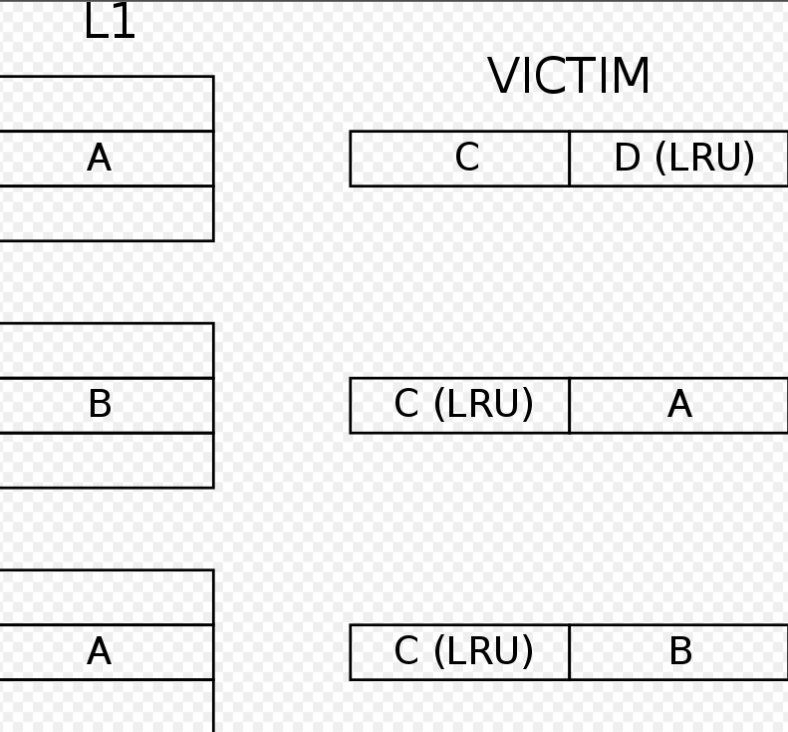
\includegraphics[width=2.28in,height=1.72in]{./media/image2.png}
	\end{Center}
\end{figure}


%%%%%%%%%%%%%%%%%%%% Figure/Image No: 1 Ends here %%%%%%%%%%%%%%%%%%%%

\par


\vspace{\baselineskip}
\setlength{\parskip}{8.04pt}
Selective Victim Cache (an improved version of victim cache)-\par

\setlength{\parskip}{6.96pt}
Another improvement in victim cache can be made by turning it into a selective victim cache. In the simple victim cache configuration, victim cache holds only those blocks evicted from the main cache as a result of replacements. In the selective victim cache configuration, some of the incoming blocks can be placed in addition to blocks resulting from replacements. When a new block is fetched to the first level cache, a prediction algorithm( not discussed in this project) is applied to determine whether the incoming block is to be placed in the main cache or the victim cache. Thus owing to this, the access time further reduces and hit rate increases, as expected.\par

{\fontsize{24pt}{28.8pt}\selectfont \textbf{\uline{Skewed Associative Cache}}\par}\par


\vspace{\baselineskip}
A Set Associative Cache and a Skewed Associative cache both have almost the same hardware complexity. The way in which Skewed and Set associative cache differ from each other is in the way of allocation of a block in their banks. The set-associative cache uses the same function (say f) to map a given memory address to a block in different banks as shown in figure1. The block chosen finally depends upon the replacement policy used. On the other hand, an N-way Skewed Associative cache also has N banks, but the block assignment in these banks is done by different functions (say f1 and f2) as shown in figure2. \par


\vspace{\baselineskip}

\vspace{\baselineskip}


%%%%%%%%%%%%%%%%%%%% Figure/Image No: 2 starts here %%%%%%%%%%%%%%%%%%%%


\begin{figure}[H]	\begin{subfigure}		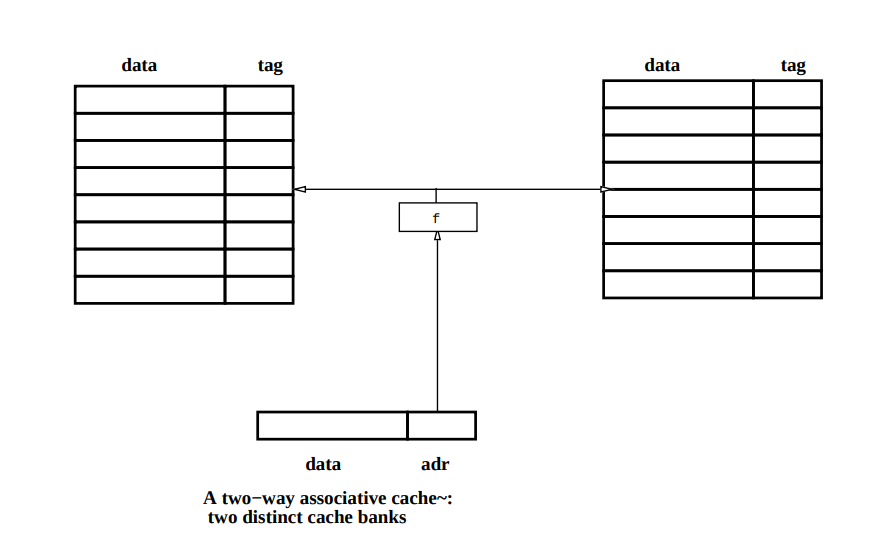
\includegraphics[width=0.45\textwidth]{./media/image3.png}
	\end{subfigure}
~	\begin{subfigure}		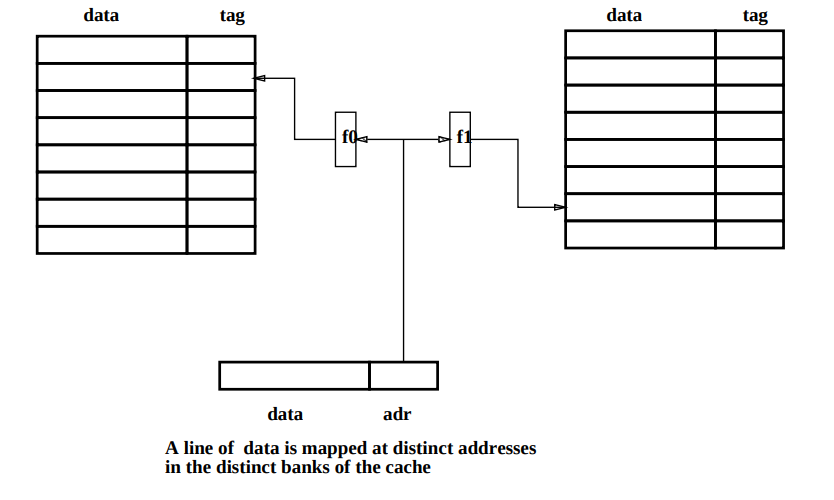
\includegraphics[width=0.45\textwidth]{./media/image1.png}
	\end{subfigure}
~
\end{figure}


%%%%%%%%%%%%%%%%%%%% Figure/Image No: 2 Ends here %%%%%%%%%%%%%%%%%%%%

\par

\tab \tab Figure 1.\tab \tab \tab \tab \tab \tab Figure 2.\par


\vspace{\baselineskip}

\vspace{\baselineskip}
\parbox{\linewidth}{Now although associativity reduces the conflict of misses, there still can be many of them even in the set-associative cache due to temporal and spatial locality. According to the principle of Skewed Associative cache, addresses in different sets should be mapped in a different way. With this the probability of conflict in all the sets at the same time reduces.}}\par


\vspace{\baselineskip}
{\fontsize{24pt}{28.8pt}\selectfont \textbf{\uline{Description\ of  Related Work}}\par}\par


\vspace{\baselineskip}
\textbf{A. }Introduced a new multi-bank cache organization: the skewed-associative cache A two-way skewed-associative cache has the same hardware complexity as a two-way set-associative cache, yet simulations show that it typically exhibits the same hit ratio as a four-way set-associative cache with the same size. Then skewed-associative caches must be preferred to set-associative caches.\par


\vspace{\baselineskip}
\textbf{B. }In this paper, we show that the recently proposed four-way skewed associative cache yields very stable execution times and good average miss ratios on blocked algorithms. As a result, execution time is faster and much more predictable than with conventional caches. As a result of its better comportment, it is possible to use larger blocks sizes with blocked algorithms, which will furthermore reduce blocking overhead costs.\par


\vspace{\baselineskip}
\textbf{C.\  }This review paper proposed the technique this technique is very useful to reduce the miss rate in cache memory. In the proposed technique the direct-mapped cache is added with a small associative cache known as a victim cache. A line removed from the direct-mapped is temporarily stored in the victim cache. \par


\vspace{\baselineskip}
\textbf{D. }This paper gave an improvement of the victim cache scheme, called selective victim caching. In this scheme, incoming blocks into the first level cache are placed selectively in the main cache or a small victim cache by the use of a prediction scheme based on their past history of use. In addition, interchanges of blocks between the main cache and the victim cache are also performed selectively.\par

\setlength{\parskip}{8.04pt}
{\fontsize{24pt}{28.8pt}\selectfont \textbf{\uline{Description of the methods used to evaluate the proposed topic}}}\par}\par


\vspace{\baselineskip}
For evaluating the caches which we had implemented, we randomly generated some addresses present in our main memory (which we had made using arrays and other data structures) and accessed the data corresponding to them. In doing so, the caches are used to store chunks of data (the data stored depends upon the cache type). We noted the hit rate, miss rate, number of accesses in main memory etc, and by using these parameters, we compared all the caches.\par


\vspace{\baselineskip}
{\fontsize{24pt}{28.8pt}\selectfont \textbf{\uline{Gantt Chart}}\par}\par


\vspace{\baselineskip}


%%%%%%%%%%%%%%%%%%%% Figure/Image No: 3 starts here %%%%%%%%%%%%%%%%%%%%

\begin{figure}[H]
	\begin{Center}
		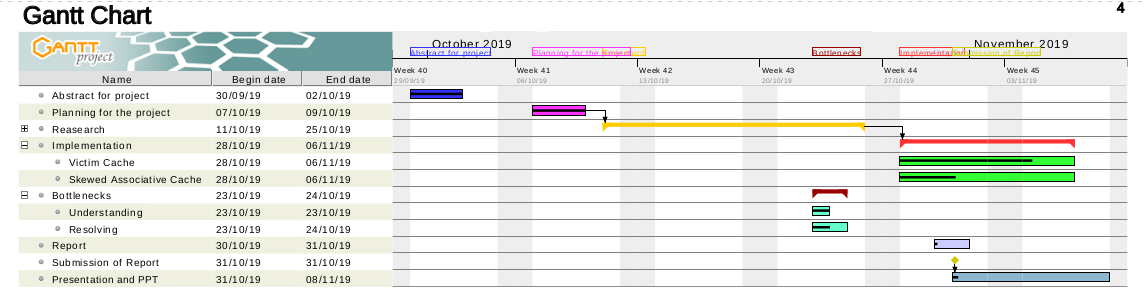
\includegraphics[width=6.55in,height=2.05in]{./media/image7.png}
	\end{Center}
\end{figure}


%%%%%%%%%%%%%%%%%%%% Figure/Image No: 3 Ends here %%%%%%%%%%%%%%%%%%%%

\par


\vspace{\baselineskip}
{\fontsize{24pt}{28.8pt}\selectfont \textbf{\textcolor[HTML]{222222}{\uline{Results And Discussion}}}}\par}\par

\parbox{\linewidth}{The two caches discussed above are two completely different ways of improving the performance of existing cache types. One type increases the physical memory space for improving the hit rate and reducing access time whereas the other cache implements an optimized method of mapping the data onto the existing physical cache memory to reduce the latency and increase the access speed of access. Therefore it would not be completely wise to compare two such different types of caches, as, for different types of input, the performance of either of the cache might be better than the other one. Nevertheless, here we have tried to compare them using a few input samples.}}\par

{\fontsize{10pt}{12.0pt}\selectfont \textbf{Victim cache output\tab \tab \tab \tab Skewed Associative cache output}\par}\par



%%%%%%%%%%%%%%%%%%%% Figure/Image No: 4 starts here %%%%%%%%%%%%%%%%%%%%


\begin{figure}[H]	\begin{subfigure}		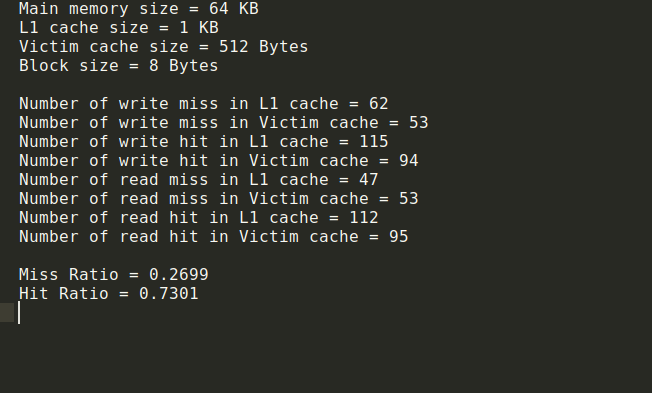
\includegraphics[width=0.28\textwidth]{./media/image4.png}
	\end{subfigure}
~	\begin{subfigure}		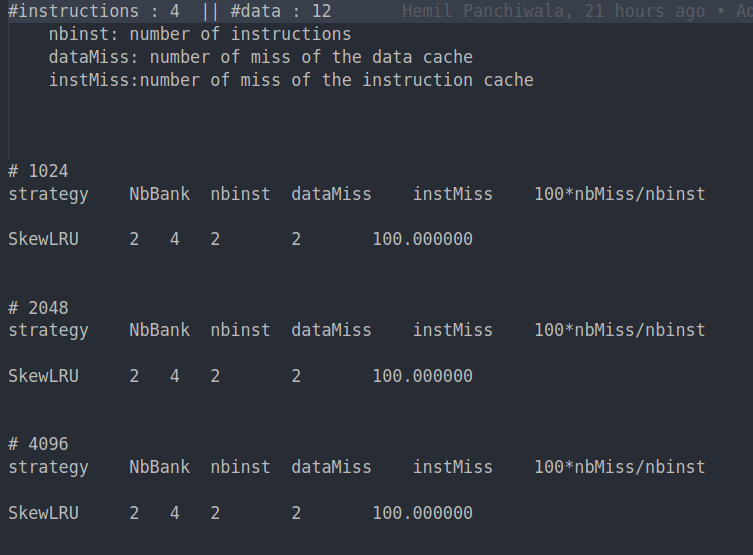
\includegraphics[width=0.28\textwidth]{./media/image6.png}
	\end{subfigure}
~	\begin{subfigure}		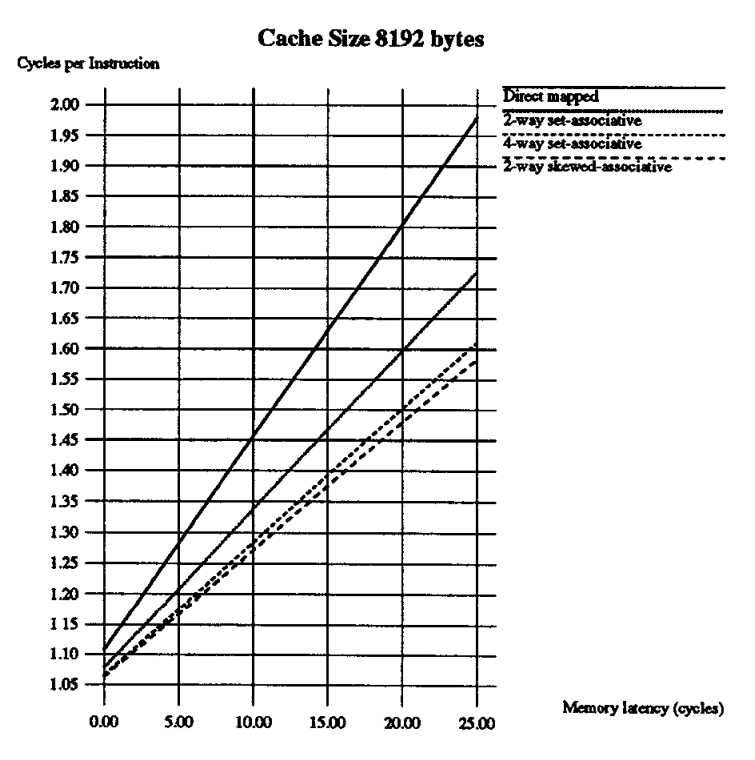
\includegraphics[width=0.28\textwidth]{./media/image5.png}
	\end{subfigure}
~
\end{figure}


%%%%%%%%%%%%%%%%%%%% Figure/Image No: 4 Ends here %%%%%%%%%%%%%%%%%%%%

{\fontsize{22pt}{26.4pt}\selectfont \ \  \par}\par

{\fontsize{10pt}{12.0pt}\selectfont \textbf{Skewed cache performance graph} \tab \tab \tab \par}\par

\tab 
\vspace{\baselineskip}
\vspace{\baselineskip}

\vspace{\baselineskip}
{\fontsize{24pt}{28.8pt}\selectfont \textbf{\uline{References}}\par}\par

A. Andre Seznec IRISA-INRIA, Campus de Beaulieu 35042 Rennes Cedex, FRANCE $``$A case for two-way skewed-associative caches$"$ .\par

\href{http://citeseerx.ist.psu.edu/viewdoc/download?doi=10.1.1.30.1042&rep=rep1&type=pdf}{\textcolor[HTML]{1155CC}{\uline{http://citeseerx.ist.psu.edu/viewdoc/download?doi=10.1.1.30.1042$\&$ rep=rep1$\&$ type=pdf}}}\par

B. $``$Skewed associativity enhances performance predictability$"$ \par

\href{https://hal.inria.fr/file/index/docid/74177/filename/RR-2499.pdf}{\textcolor[HTML]{1155CC}{\uline{https://hal.inria.fr/file/index/docid/74177/filename/RR-2499.pdf}}}\par

C. $``$High Performance Cache Architecture Using Victim Cache$"$ \par

\href{https://www.ijedr.org/papers/IJEDR1703068.pdf}{\textcolor[HTML]{1155CC}{\uline{https://www.ijedr.org/papers/IJEDR1703068.pdf}}}\par

D. $``$Selective Victim Caching: A method to improve the performance of Direct-Mapped caches$"$ \par

\href{https://ieeexplore.ieee.org/stamp/stamp.jsp?tp=&arnumber=589235}{\textcolor[HTML]{1155CC}{\uline{https://ieeexplore.ieee.org/stamp/stamp.jsp?tp=$\&$ arnumber=589235}}}\par


\vspace{\baselineskip}

\vspace{\baselineskip}

\vspace{\baselineskip}

\vspace{\baselineskip}

\printbibliography
\end{document}